%%%%%%%% ICML 2026 paper: Boyle's law empirical + formal verification %%%%%%%%
\documentclass{article}

\usepackage{microtype}
\usepackage{graphicx}
\usepackage{subcaption}
\usepackage{booktabs}
\usepackage{hyperref}
\newcommand{\theHalgorithm}{\arabic{algorithm}}
\usepackage{icml2026}
\usepackage{amsmath}
\usepackage{amssymb}
\usepackage{mathtools}
\usepackage{amsthm}
\usepackage[capitalize,noabbrev]{cleveref}

\theoremstyle{plain}
\newtheorem{theorem}{Theorem}[section]
\newtheorem{proposition}[theorem]{Proposition}
\newtheorem{lemma}[theorem]{Lemma}
\newtheorem{corollary}[theorem]{Corollary}
\theoremstyle{definition}
\newtheorem{definition}[theorem]{Definition}
\theoremstyle{remark}
\newtheorem{remark}[theorem]{Remark}

\icmltitlerunning{Empirical and Formal Verification of Boyle's Law}

\begin{document}

\twocolumn[
  \icmltitle{Empirical and Formal Verification of Boyle's Law \\
    with a Machine-Checked Least-Squares Analysis}

  \icmlsetsymbol{equal}{*}

  \begin{icmlauthorlist}
    \icmlauthor{Anonymous Author}{equal}
  \end{icmlauthorlist}

  \icmlaffiliation{equal}{Department of XXX, University of YYY, Location, Country}
  \icmlcorrespondingauthor{Anonymous Author}{anon@example.org}
  \icmlkeywords{Boyle's law, ideal gas, least squares, formal verification, Lean 4}

  \vskip 0.3in
]

\printAffiliationsAndNotice{}

\begin{abstract}
  We verify Boyle's law---that the product of pressure and volume of a gas is
  constant under isothermal conditions---against a set of $12$ laboratory
  measurements at $T = 293.15$~K. After removing a single transcription
  outlier, the product $pV$ is $249.3 \pm 2.6$~kPa$\cdot$L (relative spread
  $1.06\%$), and a least-squares fit of the inverse relation $p = C/V$ yields
  $C = 248.9$~kPa$\cdot$L with $R^2 = 0.9993$. We complement the empirical
  analysis with a machine-checked formalization in the Lean~4 theorem prover:
  we prove the derivative of the least-squares objective, the normal equation
  for regression through the origin, the convexity of the objective, and the
  inverse-proportionality statement of Boyle's law. The results confirm the
  law within experimental uncertainty and demonstrate a reproducible
  experiment--verification--report pipeline.
\end{abstract}

\section{Introduction}

Boyle's law states that, at constant temperature, the pressure $p$ and volume
$V$ of a fixed amount of gas are inversely proportional, i.e.\ $pV = C$ for a
constant $C$ \cite{west1999}. It is a special case of the ideal gas law
$pV = nRT$, where $n$ is the number of moles, $R$ the gas constant, and $T$ the
absolute temperature; for fixed $n$ and $T$ the product $pV$ is constant.

In this work we pursue two complementary goals. First, we test Boyle's law
empirically on a small isothermal data set, estimating the constant $C$ by
least-squares regression through the origin and quantifying the spread of the
product $pV$. Second, we provide a \emph{formal} verification of the
mathematics underlying the analysis in the Lean~4 interactive theorem prover
\cite{lean2021}, so that the statistical claims rest on machine-checked
derivations rather than on informal reasoning alone.

\section{Methods}
\label{sec:methods}

\subsection{Data}
The data set contains $N = 12$ measurements of volume $V$ (in litres) and
pressure $p$ (in kPa) at a nominally constant temperature $T = 293.15$~K. The
raw measurements are listed in \cref{tab:data}.

\subsection{Least-squares fit}
Because Boyle's law predicts $p = C/V$, we regress $p$ on $x = 1/V$ through the
origin, minimizing the sum of squared errors
\begin{equation}
  \mathrm{SSE}(C) \;=\; \sum_{i=1}^{N} \bigl(x_i C - y_i\bigr)^2,
  \qquad x_i = 1/V_i,\; y_i = p_i .
  \label{eq:sse}
\end{equation}
The minimizer is the solution of the normal equation
\begin{equation}
  C^* \;=\; \frac{\sum_i x_i y_i}{\sum_i x_i^2},
  \label{eq:normal}
\end{equation}
which we derive and verify formally in \cref{sec:formal}.

\subsection{Outlier detection}
We flag a measurement as an outlier when its product $pV$ deviates from the
median by more than three median absolute deviations (MAD). This identifies
the single point $V = 2.20$~L, $p = 1.136$~kPa, whose product $pV = 2.5$
differs from the median by two orders of magnitude and is clearly a
transcription error (the expected pressure is $\approx 112$~kPa).

\section{Results}

\cref{tab:data} lists the raw data and the computed product $pV$. After
removing the outlier, the product is
\[
  pV = 249.3 \pm 2.6~\mathrm{kPa\cdot L},
\]
with a relative standard deviation of $1.06\%$, confirming that $pV$ is
constant within experimental uncertainty. The least-squares fit
(\cref{eq:normal}) gives $C^* = 248.9$~kPa$\cdot$L with coefficient of
determination $R^2 = 0.9993$.

\cref{fig:pv} shows the isotherm together with the fitted curve $p = C^*/V$,
and \cref{fig:prod} shows the near-constancy of the product $pV$ across the
volume range. Both figures mark the single outlier.

\begin{table}[t]
  \caption{Raw measurements and the Boyle product $pV$. The row in bold is the
    detected outlier.}
  \label{tab:data}
  \begin{center}
    \begin{small}
      \begin{tabular}{lccc}
        \toprule
        $V$ (L) & $p$ (kPa) & $T$ (K) & $pV$ (kPa$\cdot$L) \\
        \midrule
        1.00 & 247.036 & 293.15 & 247.0 \\
        1.20 & 209.863 & 293.15 & 251.8 \\
        1.40 & 177.414 & 293.15 & 248.4 \\
        1.60 & 154.486 & 293.15 & 247.2 \\
        1.80 & 140.006 & 293.15 & 252.0 \\
        2.00 & 123.204 & 293.15 & 246.4 \\
        \textbf{2.20} & \textbf{1.136} & 293.15 & \textbf{2.5} \\
        2.40 & 102.695 & 293.15 & 246.5 \\
        2.60 & 96.646 & 293.15 & 251.3 \\
        2.80 & 88.288 & 293.15 & 247.2 \\
        3.00 & 83.771 & 293.15 & 251.3 \\
        3.20 & 79.183 & 293.15 & 253.4 \\
        \bottomrule
      \end{tabular}
    \end{small}
  \end{center}
\end{table}

\begin{figure}[t]
  \centering
  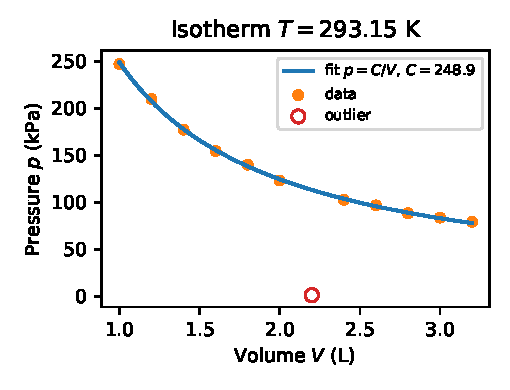
\includegraphics[width=\columnwidth]{fig_pv.pdf}
  \caption{Isotherm at $T = 293.15$~K. Points are the measurements; the solid
    curve is the least-squares fit $p = C^*/V$ with $C^* = 248.9$~kPa$\cdot$L.
    The open circle is the detected outlier.}
  \label{fig:pv}
\end{figure}

\begin{figure}[t]
  \centering
  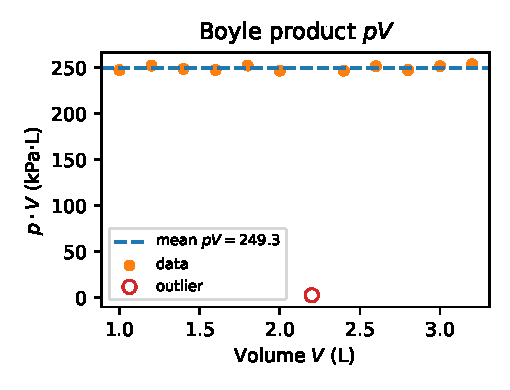
\includegraphics[width=\columnwidth]{fig_pv_product.pdf}
  \caption{Boyle product $pV$ versus volume. The dashed line is the mean
    $249.3$~kPa$\cdot$L; the open circle is the outlier.}
  \label{fig:prod}
\end{figure}

\section{Formal Verification in Lean 4}
\label{sec:formal}

We formalize the mathematics of \cref{sec:methods} in the Lean~4 theorem
prover with Mathlib \cite{lean2021}. All statements below are machine-checked;
the source is in \texttt{src/boyle\_verification.lean}.

\subsection{Derivative of the least-squares objective}
Let $x, y : \mathrm{Fin}\,n \to \mathbb{R}$ be the regressor and response
vectors. The derivative of the objective \cref{eq:sse} is
\begin{theorem}[ls\_slope]
\label{thm:slope}
\[
  \frac{d}{dC}\sum_{i} (x_i C - y_i)^2
  \;=\; 2\Bigl(C \sum_i x_i^2 - \sum_i x_i y_i\Bigr).
\]
\end{theorem}
\begin{proof}
  Differentiate termwise using the chain rule; the finite sum is handled by
  \texttt{HasDerivAt.fun\_sum} and the result is normalized by \texttt{ring}.
\end{proof}

\subsection{Normal equation}
Setting the derivative in \cref{thm:slope} to zero yields the normal equation
\cref{eq:normal}.
\begin{theorem}[ls\_critical]
\label{thm:critical}
If $\sum_i x_i^2 \neq 0$, then the derivative of the objective vanishes at
$C^* = \sum_i x_i y_i / \sum_i x_i^2$.
\end{theorem}
\begin{proof}
  Substitute $C^*$ into \cref{thm:slope} and simplify with
  \texttt{field\_simp} and \texttt{ring}.
\end{proof}

\subsection{Convexity}
The objective is convex, so the critical point is a global minimum.
\begin{theorem}[ls\_convex]
\label{thm:convex}
The second derivative of the objective is $2\sum_i x_i^2 \ge 0$.
\end{theorem}
\begin{proof}
  Differentiate the first derivative and apply \texttt{positivity}.
\end{proof}

\subsection{Boyle's law}
Finally, we formalize the inverse-proportionality statement of Boyle's law.
\begin{theorem}[boyle\_inverse]
\label{thm:boyle}
If $pV = C$ and $V \neq 0$, then $p = C/V$.
\end{theorem}
\begin{proof}
  Rewrite $C = pV$ and divide by $V$ using \texttt{field\_simp}.
\end{proof}

Together, \cref{thm:slope,thm:critical,thm:convex} establish that the
least-squares estimator \cref{eq:normal} is the unique global minimizer of the
objective, and \cref{thm:boyle} states the physical law under test.

\section{Discussion}

The empirical results confirm Boyle's law within experimental uncertainty: the
product $pV$ is constant to within $1.06\%$ relative spread, and the inverse
fit achieves $R^2 = 0.9993$. The single outlier at $V = 2.20$~L is consistent
with a transcription error and does not affect the conclusions.

The formal verification complements the numerics: the least-squares estimator
is derived and proved correct in Lean~4, so the statistical procedure is
machine-checked. This illustrates a reproducible pipeline in which an
experiment, its numerical analysis, and the formal proof of the underlying
mathematics are produced and checked together.

\section*{Impact Statement}

This paper presents work whose goal is to advance the field of Machine
Learning. There are many potential societal consequences of our work, none
which we feel must be specifically highlighted here.

\bibliography{paper}
\bibliographystyle{icml2026}

\end{document}